\documentclass[a4paper,10pt,twocolumn,uplatex]{jsarticle}
\usepackage{style/nislab,style/resume}

%---------------------------------------------------------------------
% レジュメ種別・日付設定(要変更)
% \type{} 1:修士論文諮問会 2:卒業論文発表会 3:月例発表会 4:研究室合同発表会
%---------------------------------------------------------------------
\type{3}
\year{2023}
\month{6}
\date{10}

%---------------------------------------------------------------------
% ページ番号設定(要変更)
%---------------------------------------------------------------------
\setcounter{page}{5}

%---------------------------------------------------------------------
% 変更不要
%---------------------------------------------------------------------
\begin{document}

%---------------------------------------------------------------------
% タイトル作成部分(要変更)
% \maketitle{タイトル}{title}{名前}{name}
%---------------------------------------------------------------------
\maketitle{SDNを利用したQoS予測・予約によるV2X通信の信頼性向上}
{Improvement of V2X Communication Reliability\\by QoS Prediction \& Reservation Using SDN}
{国本 典晟}
{Tensei KUNIMOTO}

%---------------------------------------------------------------------
\section{はじめに}
車両に搭載されたセンサで認識できる範囲は限定的であるため,周囲の車両や路側機のセンサが認識した情報を通信により共有することで,交通の安全性や効率の向上を目指す協調型自動運転の研究が行われている\cite{Cooperative}.
各車両や路側機が収集したセンサデータをサーバ上で集約し,統合した情報を車両に配信することで,車両は自車両の搭載センサでは認識できない情報を取得することができる.
センサデータを集約・統合するサーバとしてインターネット上のクラウドサーバを利用する場合,膨大な数の車両からのデータをインターネットを介して扱うため,処理負荷や通信遅延が増大し,衝突危険警告や合流調停などの遅延要件を満たすことができないことが懸念される.
そこで,車両とクラウドサーバの間に地理的に分散配置されたエッジサーバを利用することで,処理負荷の分散や通信遅延の軽減が期待されている\cite{MEC}.\par
エッジサーバは自身が管轄するエリア内に存在する車両や路側機と基地局を介した通信によりデータを集約し,協調型自動運転のための処理を行う.
しかし,エッジサーバまでの通信帯域で収容可能な台数以上の車両がエリア内に集中した場合,通信帯域が逼迫し,一部または全ての車両とエッジサーバの通信の遅延が増大し,QoS(Quality of Service)を保証することができないことが懸念される\cite{QoS}.
QoSを保証できない場合,車両は情報を遅延要件内に取得可能か判断できないまま協調型自動運転を試みることになり,安全性や効率の点で重大な問題となる.
本研究では,ソフトウェアを介してネットワークを一元管理するSDN(Software-Defined Networking)を利用して,QoSの予測・予約を行うことで車両の通信のQoSを保証することを提案する.

%---------------------------------------------------------------------
\section{提案手法}
\subsection{SDNを利用したネットワーク}
% エッジサーバの分散配置については様々な議論がなされているが、本研究では1台のエッジサーバが複数の基地局の通信範囲を対象エリアとするネットワークを考える.
SDNではネットワークを構成する機器をSDNコントローラと呼ばれる制御装置を用いて集中管理を行う.
本研究では,\figref{fig:SDNnetwork}のように,複数のエッジサーバを管理するSDNコントローラを考える.
SDNコントローラは地図情報に合わせて,管理するエッジサーバの位置,対象エリア,利用可能な通信帯域の情報を保持する.
車両,基地局,エッジサーバが行う通信はSDNコントローラによって管理されており,車両,基地局,エッジサーバはSDNコントローラと管理に必要な情報の通信を行う.
管理に必要な通信のための通信帯域は常に確保されているものとする.

\begin{figure}[t]
	\begin{centering}
    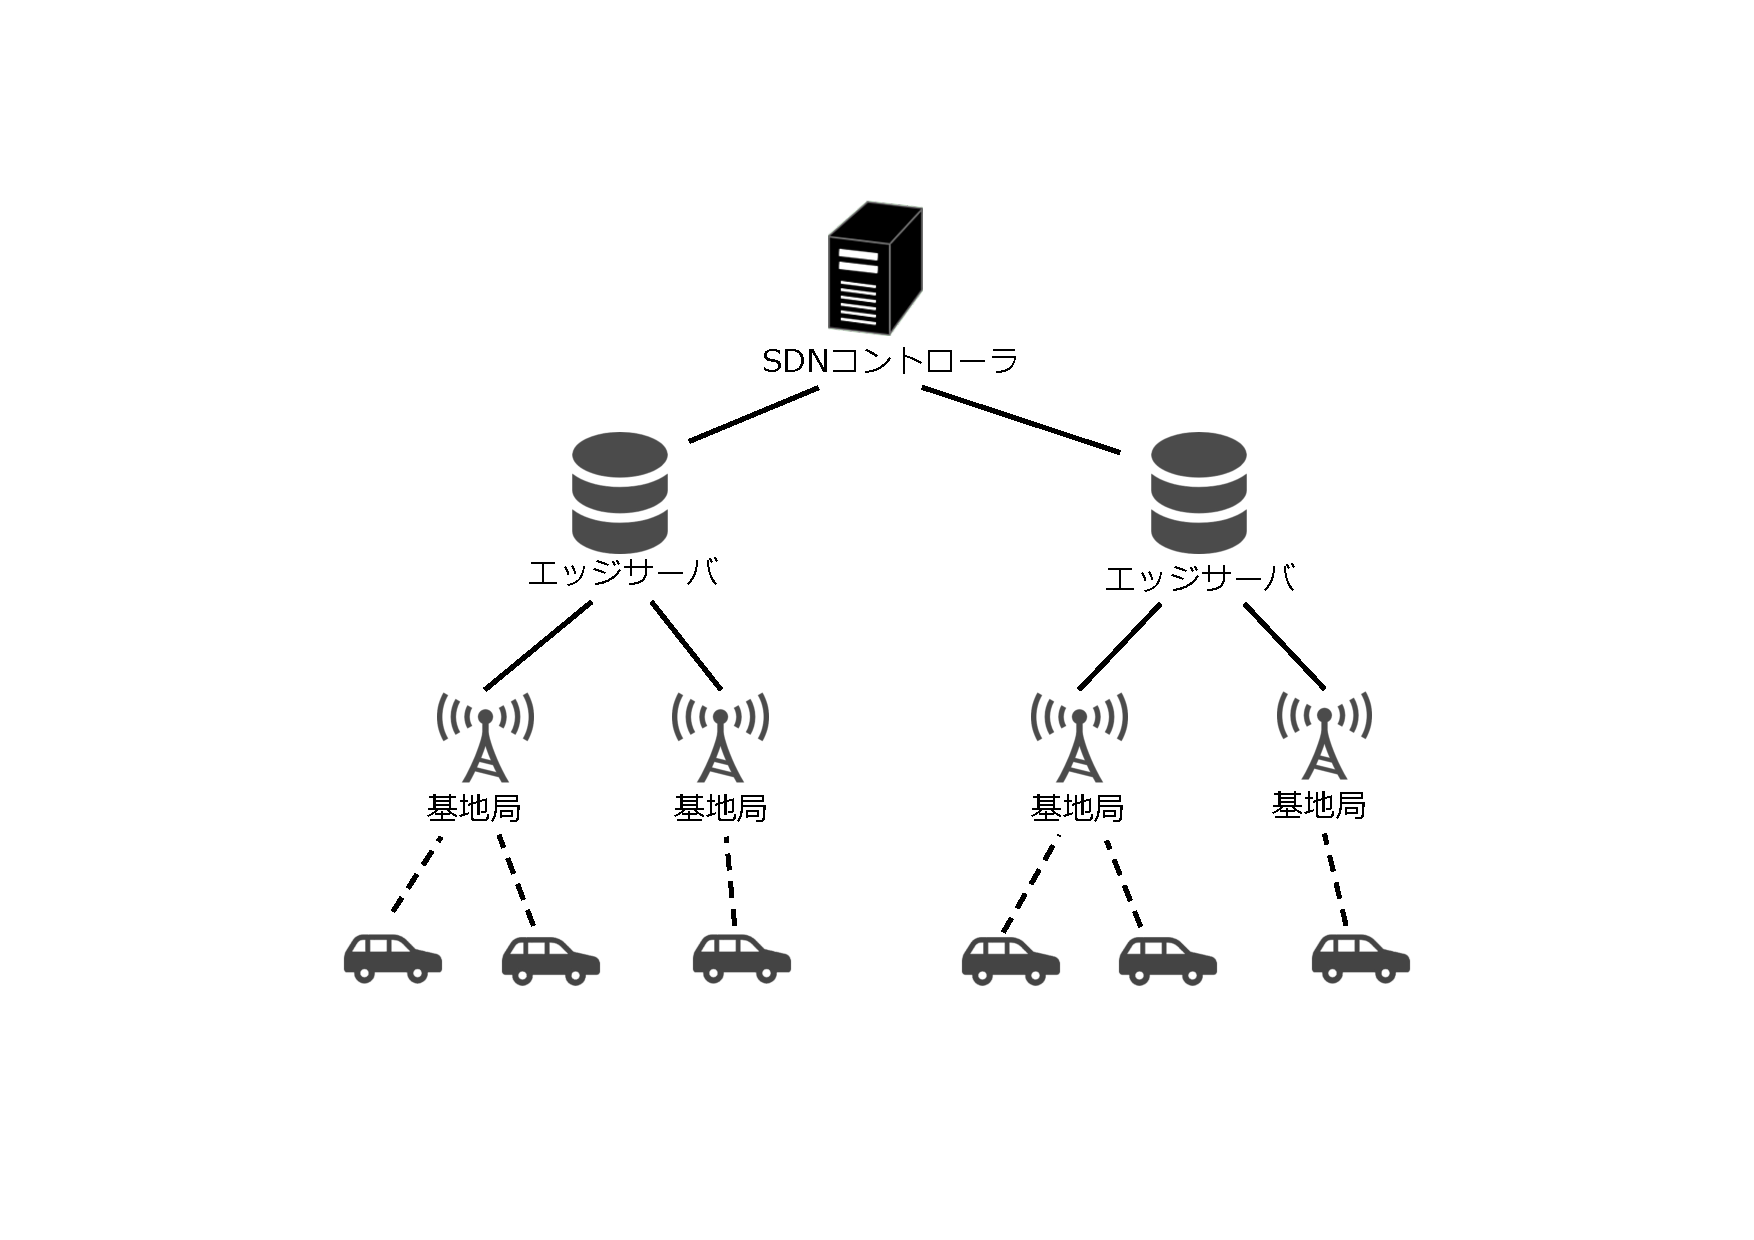
\includegraphics[width=0.94\linewidth]{img/202306_SDNnetwork.pdf}
    \caption{SDNを利用したネットワーク}
    \label{fig:SDNnetwork}
    \end{centering}
\end{figure}

%---------------------------------------------------------------------
\subsection{QoS予測}
\label{QoSprediction}
エッジサーバまでの通信のQoSが保証されるかを事前に予測するため,SDNコントローラは\figref{fig:QoSprediction}の手順でQoS予測を行う.
初めに,SDNコントローラは管理エリア内の車両から車両IDと移動計画を集約する.
次に,SDNコントローラは集約した情報から,ある時刻における各基地局の通信エリア内の車両の総台数を想定する.
最後に,想定した車両の総台数と保持している利用可能な通信帯域の情報から,全ての車両の通信のQoSを保証できるかを判断する.
なお,ここでは全ての車両が協調型自動運転のために同じデータサイズの通信を行うものとする.
以上のQoS予測のための手順は定期的に行われ,SDNコントローラは常に一定時刻後のQoSを予測する.

\begin{figure}[t]
	\begin{centering}
    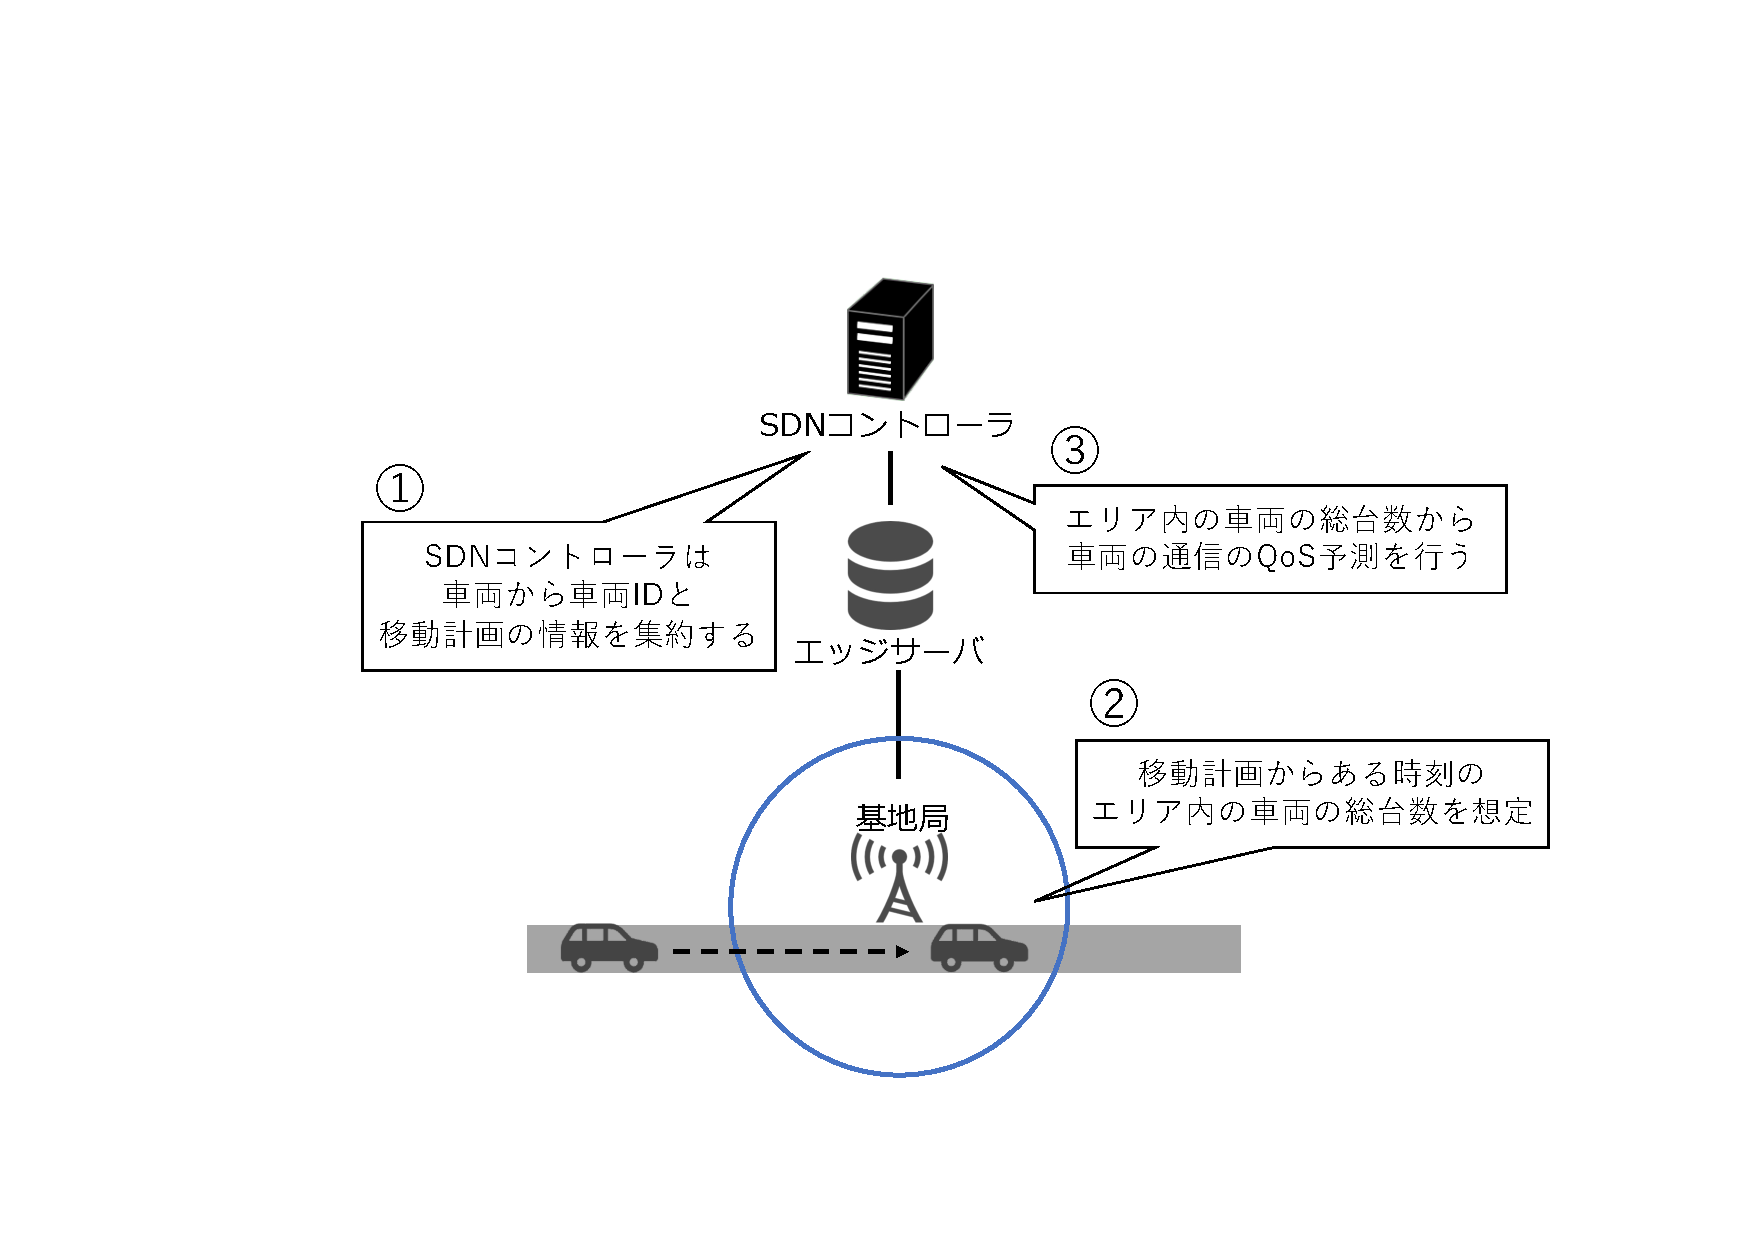
\includegraphics[width=\linewidth]{img/202306_QoSprediction.pdf}
    \caption{QoS予測の手順}
    \label{fig:QoSprediction}
    \end{centering}
\end{figure}

%---------------------------------------------------------------------
\subsection{QoS予約}
QoSが保証できない場合,車両はある時刻において協調型自動運転に必要な情報を取得可能かを事前に判断できない.
そこで,事前にSDNコントローラからある時刻において各車両に通信可能か否かを通知することで,QoSの予約を行う.
QoS予測の結果,全ての車両の通信のQoSが保証できると判断した場合,SDNコントローラは各車両にある時刻でのQoSが予約されていることを通知する.
一方,全ての車両の通信のQoSの保証はできないと判断した場合,SDNコントローラは利用可能な通信帯域でQoSが保証できる台数分の車両にQoSが予約されることを通知し,残りの車両にはQoSが予約されないことを通知する.
これにより,全ての車両は移動計画の通りに走行した場合に,ある時刻において協調型自動運転のための通信のQoSが保証されているかを事前に把握することができる.
QoS予測同様,QoS予約も定期的に行われ,車両は常に一定時刻後の通信のQoSが予約されているか否かを把握する.
QoSを予約しない車両の選択方法やそれらの車両のQoSの保証の方法については様々なものが考えられるが,本研究では対象外とする.

%---------------------------------------------------------------------
\section{シミュレーションによる評価}
\label{simulation}
提案手法を評価するにあたり,ネットワークシミュレータであるNS-3を用いて,\figref{fig:model}に示すような車両移動モデルでシミュレーションを行う.
4つのT字路交差点にはそれぞれ交差点とその周囲を通信エリアとする基地局が設置されており,基地局を2つずつ管轄するエッジサーバが2つあり,モデル内の全ての車両,基地局,エッジサーバを管理するSDNコントローラが1つある.
SDNコントローラは定期的に一定時刻後のQoS予測と各車両へのQoS予約の通知を行う.
全ての車両はシミュレーション中一定速度でランダムに移動し,移動中は定期的にQoS予測・予約に必要な情報な通信を行う.
また,車両はQoSが予約されていると通知された場合には協調型自動運転のための通信を行い,QoSが予約されないと通知された場合には協調型自動運転のための通信を行わない.\par
QoS予測・予約の有効性を検証するため,車両とエッジサーバ間の協調型自動運転のための通信の遅延およびパケットロス率の評価を行う.
車両台数を変化させて,提案手法におけるQoSが予約された車両とされていない車両での通信の遅延およびパケットロス率を測定する.
QoS予測・予約を行わず全ての車両が常に協調型自動運転のための通信を行う場合の通信の遅延およびパケットロス率と比較することで,車両が集中した場合の車両の通信のQoSを評価する.

\begin{figure}[t]
	\begin{centering}
    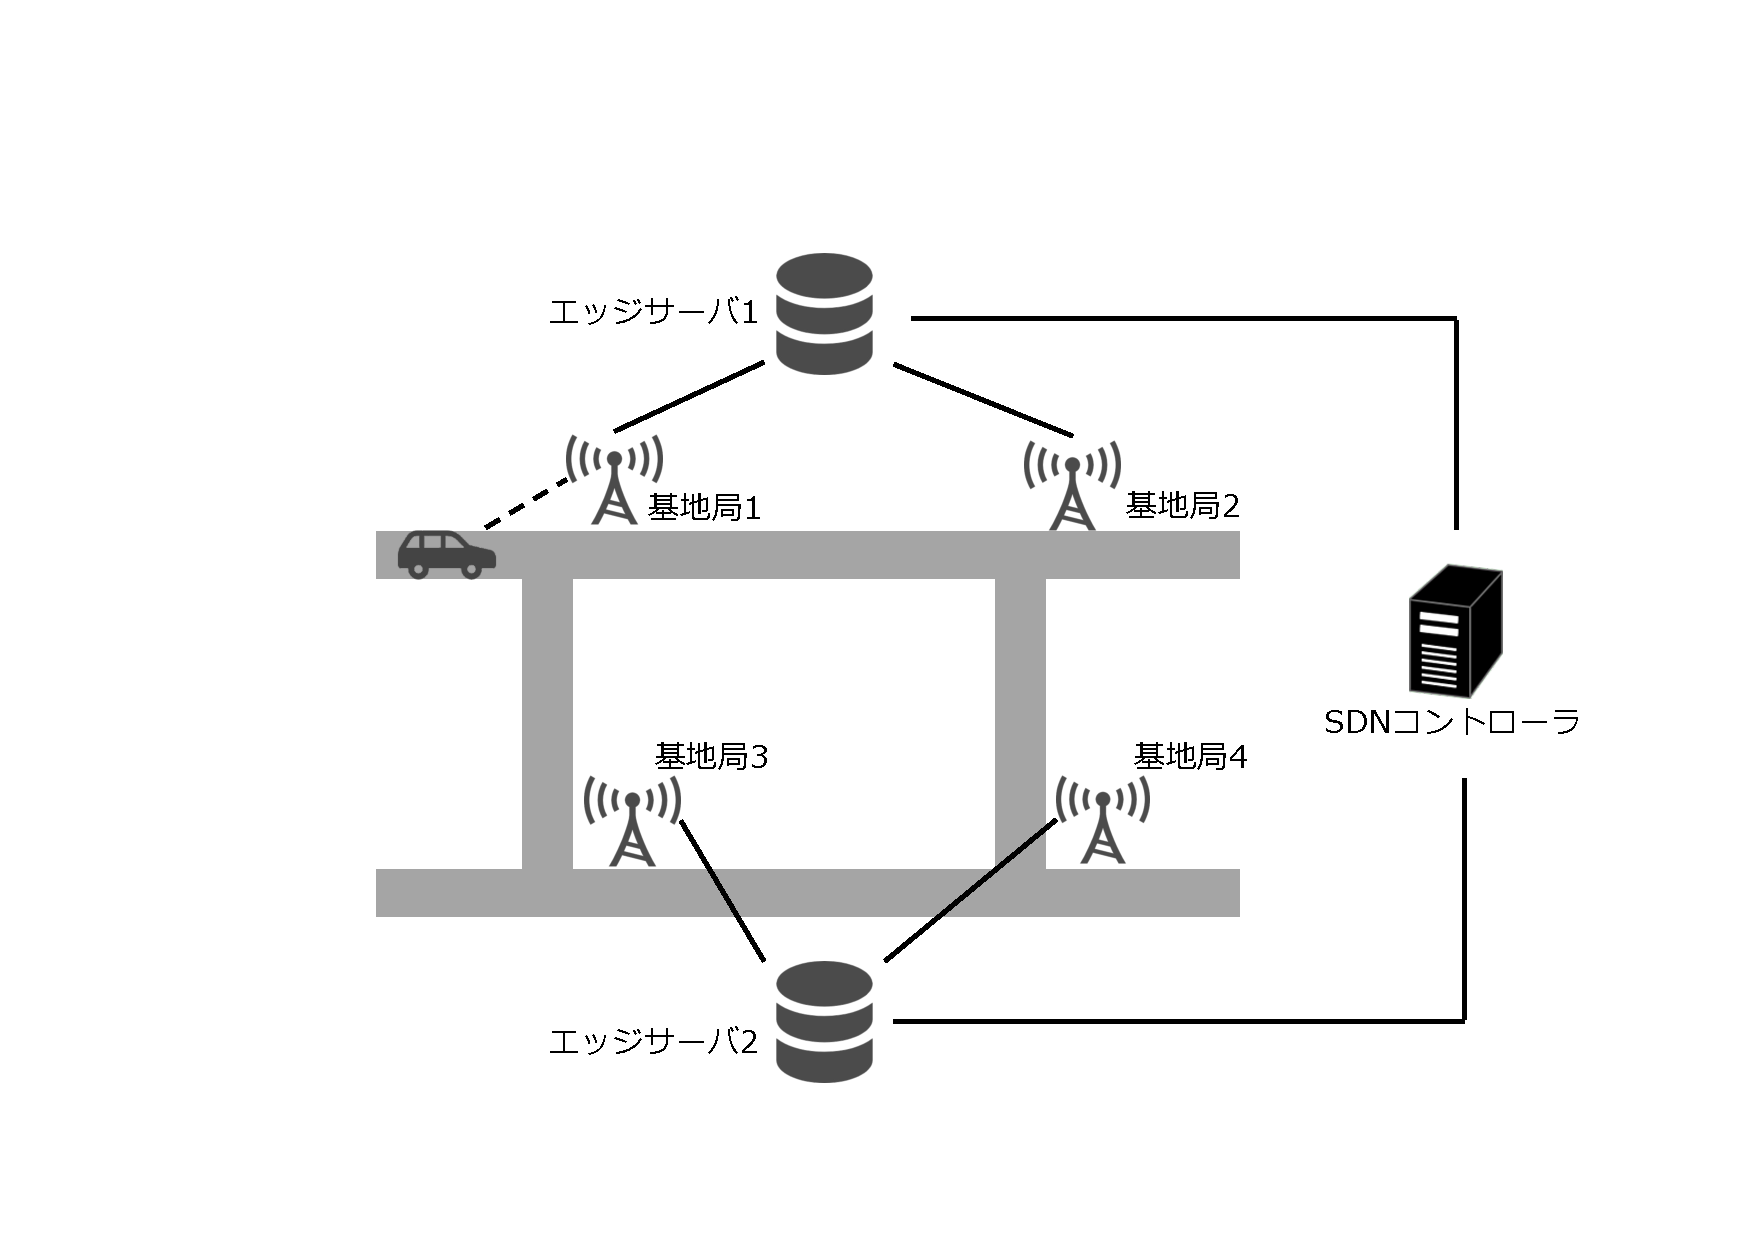
\includegraphics[width=\linewidth]{img/202306_simulationModel.pdf}
    \caption{シミュレーションモデル}
    \label{fig:model}
    \end{centering}
\end{figure}

%---------------------------------------------------------------------
\section{まとめと今後の課題}
協調型自動運転においてエッジサーバの利用が検討されているが,エッジサーバまでの利用可能な通信帯域で収容可能な台数以上の車両が集中した場合に,一部または全ての車両が遅延要件内に協調型自動運転のための情報を取得できないことが懸念される.
本研究では,SDNを利用して車両の移動計画を集約し,基地局の通信エリア内の一定時刻後の車両の集中状況を想定することで,全ての車両の通信のQoSを保証できるかを予測し,その結果を車両に通知することでQoSを予約することを提案した.
今後はネットワークシミュレーションによって,提案手法を用いて車両の通信のQoSを保証できるかを評価する.\par
本研究では,1つのSDNコントローラの管理エリア内で完結するQoS予測・予約について検討したが,実際には他のSDNコントローラの管理エリアから進入する車両が存在するため,SDNコントローラ間で入出車両を共有する仕組みが必要であると考えている.
また,基地局の通信エリアのハンドオーバを考慮したQoS予測や,QoS予約に付随する車両の移動計画や通信の制御についても検討する必要があると考えている.

%---------------------------------------------------------------------
% Bibliography(参考文献)
%---------------------------------------------------------------------
% thebibliography を利用する場合は以下を使用
\footnotesize{
  \begin{thebibliography}{99}
    \bibitem{Cooperative} 菅沼英明,ITS・自動運転の動向と今後,電子情報通信学会通信ソサイエティマガジン,Vol.15,No.2,pp.102-108,2021.
    \bibitem{MEC} Fuhui Zhou, Rose Qingyang Hu, Zan Li and Yuhao Wang, Mobile edge computing in unmanned aerial vehicle networks, \textit{IEEE Wireless Communications}, Vol.27, No.1, pp.140-146, 2020.
    % ETSI, Multi-access Edge Computing (MEC); Study on MEC Support for V2X Use Cases, 2018.
    \bibitem{QoS} Ignacio Soto, Maria Calderon, Oscar Amador and Manuel Uruena, A survey on road safety and traffic efficiency vehicular applications based on C-V2X technologies, \textit{Vehicular Communications}, Vol.33, No.100428, 2022.
    % Kousaridas A., Schimpe A., Euler S., et al, 5G cross-border operation for connected and automated mobility: Challenges and solutions, MDPI Future Internet, vol.12, no.1, 2020.
  \end{thebibliography}
}

% BibTex を利用する場合は以下を使用(初めての人には難しいかも)
% \bibliographystyle{junsrt}
% \bibliography{myref}

%---------------------------------------------------------------------
\end{document}
%---------------------------------------------------------------------
